\ylDisplay
{}% Problem name
{2021}% Year
{mcq}% Round (mcq, theory, experiment)
{2}% Problem nr.
{physics}% Subject (physics, chemistry, biology)
{}% Difficulty (1-3)
{
% Syl:
\ifStatement
A light beam is travelling from vertically infinite region 1 to vertically infinite region 4 (refer to figure). The refractive indexes in regions 1, 2, 3, 4 are \num{1.62}, \num{1.60}, \num{1.55}, and \num{1.50}, respectively. The sin of angle of incidence $\theta$ for which the beam just misses entering region 4 is
\begin{center}
  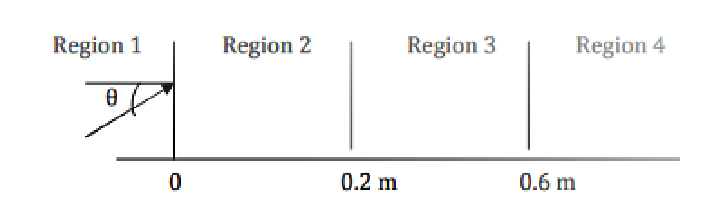
\includegraphics[width=.7\linewidth]{2021-mcq-02-p}
\end{center}

\fi


\ifOption1
$\frac{\num{1.50}}{\num{1.55}}$
\fi


\ifOption2
$\frac{\num{1.50}}{\num{1.62}}$
\fi


\ifOption3
$\frac{\num{1.60}}{\num{1.62}}$
\fi


\ifOption4
$\frac{\num{1.55}}{\num{1.60}}$
\fi


\ifHint

\fi


\ifSolution

\fi


\ifEstStatement
% Problem name:

\fi


\ifEstOption1

\fi


\ifEstOption2

\fi


\ifEstOption3

\fi


\ifEstOption4

\fi


\ifEstHint

\fi


\ifEstSolution

\fi
}
